
%HW14.tex
%Fourteenth Homework -- Math 629 
%
%  The percent sign is a comment character
%
%%%%%%%%%%%%%%%%%%%%%%%%%%%%%%%%%%%%%%%%%%%%%%%%%%%%%%%%%%%%%%%%%%%%%%%%%%%%%%%%%%
%
%   Look these up on line.  The first sets the type of document, and the next are for mathematics symbols, graphics and color
%
\documentclass[12pt]{article}
\usepackage{amssymb,amsmath}
\usepackage{graphicx}
\usepackage[usenames,dvipsnames,svgnames,table]{xcolor}
\usepackage{multirow}   % This is for more control over tables
%%%%%%%%%%%%%%%%%%%%%%%%%%%%%%%%  Layout     %%%%%%%%%%%%%%%%%%%%%%%%%%%%%%%%%%%%%%
\usepackage{vmargin}
\setpapersize{USletter}
\setmargrb{2cm}{0cm}{2cm}{1cm} % --- sets all four margins LTRB

%%%%%%%%%%%%%%%%%%%%%%%%%%%%%%%%%%%%%%%%%%%%%%%%%%%%%%%%%%%%%%%%%%%%%%%%%%%%%%%%%
\begin{document}
\LARGE 
\noindent
{\color{Maroon}History of Mathematics \hfill Math 629}\vspace{2pt}\\
\large
Fourteenth Homework: \hfill 23 April 2024\\
Due Monday 29 April 2024.
\normalsize\vspace{10pt}

To hand in: We are using Gradescope for homework submission.

\begin{enumerate}


\item  {[10]}  Exercise 24.2.1
    
\item  {[10]}  Exercise 24.2.2
    
\item  {[10]}  Exercise 25.5.2
    
\item  {[10]}  Exercise 25.5.4
    
\item  {[10]}  Exercise 25.5.5

\item {[20]} After building your model of the 4-cube, complete the worksheet (on the next sheet of paper).

\item {[20]} Write a paragraph about what you we learned from the project. 
  
\end{enumerate}

\newpage


\begin{center}
{\color{Maroon}\underline{{\Large\sf Cubes Worksheet}}}
\end{center}

\noindent\hspace{-8pt}
\begin{tabular}{||c|c|c|c|c|c|c|c|c||}\hline\hline
\Large $d$ & $d$-Cube&\quad \ $v$\quad \ &\quad \ $e$\quad \ &\ \quad $f_2$\quad \ &\quad $f_3$\quad\  
           &\quad $f_4$\quad\ &\quad $f_5$\quad\ \ \raisebox{-5pt}{\rule{0pt}{20pt}}&\quad\ 
           Sum\quad\  \\\hline
\Large 0 & 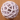
\includegraphics{pictures/point.eps}&&&&&&&\raisebox{-15pt}{\rule{0pt}{35pt}}\\\hline
\Large 1 & 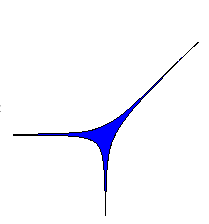
\includegraphics{pictures/line.eps}&&&&&&&\raisebox{-15pt}{\rule{0pt}{35pt}}\\\hline
\Large 2 & \includegraphics{pictures/square.eps}&&&&&&&\raisebox{-10pt}{\rule{0pt}{25pt}}\\\hline
\Large 3 & \includegraphics{pictures/cube.eps}&&&&&&&\raisebox{-10pt}{\rule{0pt}{25pt}}\\\hline
\Large 4 & [Your Model] &&&&&&&\raisebox{-20pt}{\rule{0pt}{50pt}}\\\hline
\Large 5 & [Your Mind] &&&&&&&\raisebox{-20pt}{\rule{0pt}{50pt}}\\\hline
\Large $n$ & [Your Mind] &&&&&&&\raisebox{-20pt}{\rule{0pt}{50pt}}\\\hline
\Large $d$ & $d$-Cube&\quad \ $v$\quad \ &\quad \ $e$\quad \ &\ \quad $f_2$\quad \ &\quad $f_3$\quad\  
                 &\quad $f_4$\quad\ &\quad $f_5$\quad\ \ \raisebox{-5pt}{\rule{0pt}{20pt}}&\quad\ 
           Sum\quad\ \\\hline\hline
%\Large $d$ & &&&&&&\\\hline
\end{tabular}\vspace{3pt}

\noindent\large
  What is the sum of the face numbers of a $d$-cube? \newline
  What about its face numbers?
  {\color{Blue}The second question is hard.}\bigskip

This is a picture of the Schlegel diagram of the four-dimensional cube.  
It is different from the model you just made.
\[
   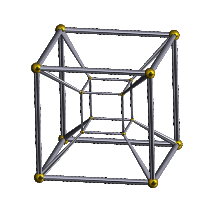
\includegraphics[height=180pt]{pictures/Schlegel-4Cube.eps}
\]


\end{document}


%
%   Parallelepiped model
%
%

